\begin{figure}[th]
    \centering
    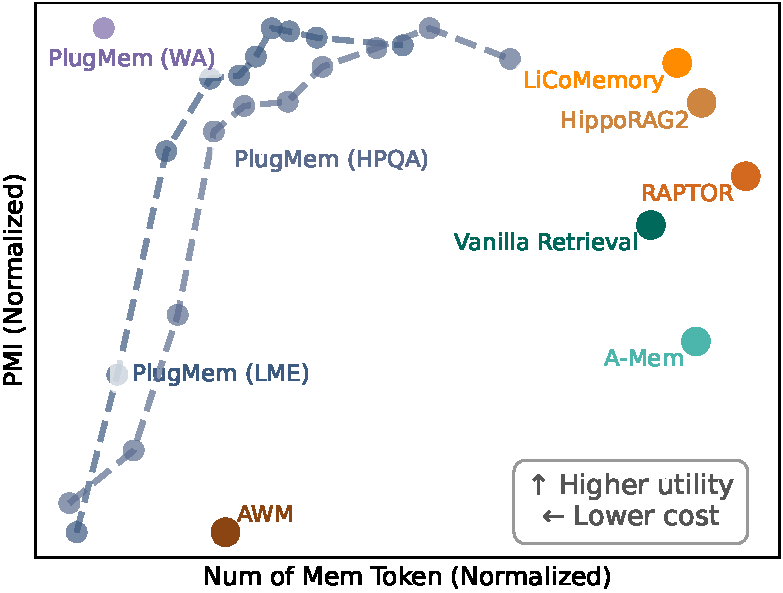
\includegraphics[width=0.4\textwidth]{Figures/hero_figure.pdf} 
    \caption{\label{fig:hero_figure}
    A utility–cost visualization of agentic memory approaches.\footnotemark \textbf{\mbox{\plugmem}, evaluated unchanged across heterogeneous benchmarks requiring processing multiple memory types, achieves the highest decision-making utility of memory at the lowest agent-side memory cost.}
    }
\end{figure}

\footnotetext{Each point corresponds to a memory method evaluated on at least one of three benchmarks, i.e., LongMemEval~\citep{wu2024longmemeval}, HotpotQA~\citep{yang2018hotpotqadatasetdiverseexplainable} and WebArena~\citep{zhou2024webarenarealisticwebenvironment}, plotted in a normalized utility–cost space to enable cross-task visualization and to accommodate baselines that are not applicable to all benchmarks. Both axes are min–max normalized, which linearly rescales values to a fixed range (e.g., $[0,1]$) while preserving relative ordering across methods. Curves are obtained by sweeping the memory token budget. The normalization is applied solely for visualization; detailed benchmark-specific analyses using raw PMI values and token numbers are reported in Section~\ref{sec:experiments} and Figure~\ref{fig:utility_cost}.}


\section{Introduction}
\begin{figure*}[ht]
    \centering
    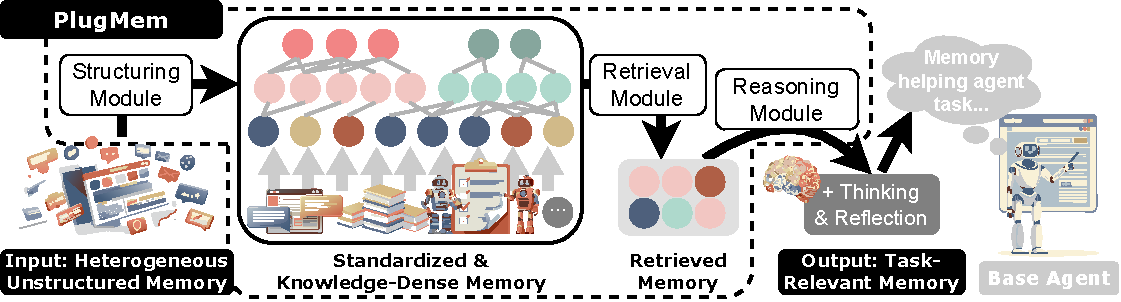
\includegraphics[width=\textwidth]{Figures/overview.pdf}
    \caption{\label{fig:overview}
    \plugmem organizes raw memory and outputs refined memory tokens to help the base agent's decision-making.
    }
\end{figure*}

Large language model (LLM) agents increasingly operate in settings that require long-term memory, where relevant information is distributed across long interaction histories and must be reused to support future decisions~\citep{Wang_2024,park2023generativeagentsinteractivesimulacra}. However, naively accumulating past interactions as raw context quickly leads to unbounded memory growth, high computational cost, and degraded performance~\citep{packer2024memgptllmsoperatingsystems,liu2023lostmiddlelanguagemodels}. To address this, many agent architectures rely on external memory modules to store and retrieve past experience.
Yet most existing memory designs tightly couple memory representation and retrieval to specific tasks or benchmarks, relying on hand-crafted heuristics for what to store and how to use it~\citep{wang2024agentworkflowmemory,gutiérrez2025ragmemorynonparametriccontinual}. While effective in narrow settings, such task-specific memory modules fail to generalize: a memory system optimized for long-horizon conversations does not readily transfer to web navigation, and vice versa. This limitation motivates the need for a \textit{task-agnostic plug-and-play} memory module that can be attached to arbitrary LLM agents without task-specific redesign, reducing per-task engineering overhead and enabling a single memory module to be reused across diverse agentic settings.


Designing such a general plugin memory module is challenging. The most straightforward task-agnostic approach is retrieval-based memory, where all past experiences are stored as raw text chunks and retrieved by relevance (optionally augmented with reasoning, as in RAG). However, this paradigm often fails in practice due to \textit{knowledge sparsity}. Memories that are truly useful for decision-making are typically condensed and abstract forms of knowledge, whereas raw memories are verbose, episodic, and dominated by low-level information. For example, when recommending recipes, an agent benefits from knowing a user’s dietary preferences and restrictions, which are compact factual propositions distilled from many interactions, rather than re-reading long conversation histories. Similarly, when shopping on a previously unseen web interface, an agent needs generalizable procedural knowledge, i.e., how to search, filter, and check out, not raw trajectories containing full-page observations with thousands of irrelevant tokens. Treating raw episodic memory as directly usable knowledge therefore imposes an unnecessary context burden and obscures the information most relevant for decision-making.

Prior work has attempted to bridge this gap by compressing or summarizing memory, but largely in task-specific ways. Memory modules are often engineered to perform well on a particular benchmark, such as conversational long-term memory or web-based agents, implicitly assuming a single dominant type of memory~\citep{wang2024agentworkflowmemory,gutiérrez2025ragmemorynonparametriccontinual}. When applied to a different task domain, these designs rarely transfer without significant task-specific modifications. This raises a key challenge: how can we design a general-purpose memory module that simultaneously supports multiple memory types and adapts to the diverse demands of agentic tasks, and evaluate it in a way that jointly reflects decision utility and agent-side cost, while allowing cross-task comparability?

To address the design side of this challenge, we ground our approach in a principled account of memory organization from cognitive science. Decades of research suggest that the human brain makes a fundamental distinction between episodic memory (detailed records of experience) and knowledge-level memory, which can be further divided into semantic memory (knowing that; factual \textit{propositions}) and procedural memory (knowing how; action-oriented \textit{prescriptions})~\citep{Tulving1972EpisodicSemantic, Squire2004MemorySystems}. Episodic memory serves as the source from which propositional and prescriptive knowledge are abstracted, while the latter forms are most directly useful for reasoning and decision-making. This perspective suggests that effective agent memory should not merely retrieve past experiences, but actively transform raw episodic memory into structured, knowledge-dense representations.

Based on these principles, we introduce a novel plugin memory module \plugmem, that performs \textit{memory-to-knowledge abstraction} and supports the unified management of multiple key memory types across agentic tasks. As shown in Figure~\ref{fig:overview}, our approach consists of: \textit{i)} a \textit{structuring module} that standardizes heterogeneous raw memories and extracts propositional and prescriptive knowledge through hierarchical abstraction, organizing them into a memory graph; \textit{ii)} a \textit{retrieval module} that selects task-relevant subgraphs; and \textit{iii)} a \textit{reasoning module} that further adapts and compresses retrieved knowledge for the base agent. Unlike conventional knowledge graphs that operate on entities and relations, our memory graph operates on \textit{knowledge units} (i.e., propositions and prescriptions) which form the fundamental units of memory access and manipulation. \plugmem can be viewed as a knowledge-centric form of GraphRAG~\citep{edge2025localglobalgraphrag} tailored for memory management, where graph nodes are knowledge rather than entities or text chunks.

Complementary to the design of a general-purpose memory module, we contribute a novel utility-cost analysis framework that enables fair comparison between different memory designs across tasks, capturing both performance improvements and memory efficiency. Specifically, we measure the \textit{information density} of memory, defined as the decision-relevant information gain provided to the base agent per memory token. We implement \plugmem and evaluate it on three heterogeneous and challenging benchmarks: long-horizon conversational question answering~\citep{wu2024longmemeval}, multi-hop knowledge retrieval over Wikipedia~\citep{yang2018hotpotqadatasetdiverseexplainable}, and web-based agent tasks~\citep{zhou2024webarenarealisticwebenvironment}. \textit{Using the same memory module implementation across all settings}, we demonstrate consistent performance gains over vanilla task-agnostic baselines and task-specific memory modules, while incurring lower agent-side memory cost, as illustrated in Figure~\ref{fig:hero_figure}.
Ablation studies further clarify the roles of different components. Since agentic memory ultimately serves decision-making, task performance is primarily determined by whether retrieval brings the most useful memory to bear at decision time. Our structuring module incrementally enhances retrieval by organizing heterogeneous experience into knowledge-centric memory units, yielding additional performance gains. Meanwhile, the reasoning module substantially improves efficiency, reducing memory token usage by one to two orders of magnitude through task-adaptive condensation. We provide illustrative benchmark examples in Appendix~\ref{app:real_benchmark_cases}. 

In summary, our contributions are fourfold:

\begin{itemize}[leftmargin=*, noitemsep, topsep=0.5pt]

    \item \textbf{Design principles:} cognitively motivated principles for task-agnostic memory in LLM agents.
    \item \textbf{Evaluation framework:} an information-theoretic measure of memory utility and efficiency.
    \item \textbf{General memory module:} a plugin memory system applicable across heterogeneous agentic benchmarks. 
    \item \textbf{Reproducibility:} released code and experimental results.
\end{itemize}
